\begin{table*}[h!]
\centering
\caption{Scenario 5 Rankings and Voting Summary}
\label{tab:s5}
\resizebox{\textwidth}{!} {
\begin{tabular}{|l|llc|}
\hline
\multirow{8}{*}{\begin{tabular}[c]{@{}c@{}}\\ 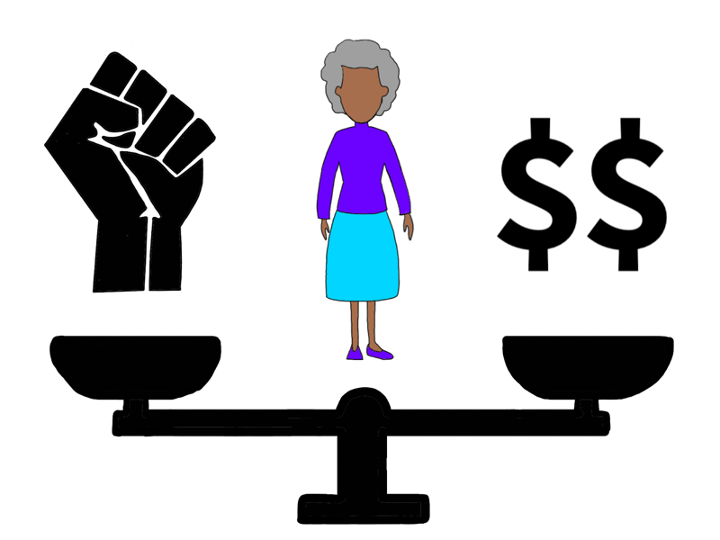
\includegraphics[width=2.75cm]{Chapters/images/marianne.png} \\ {Marianne's earnings} \\ {were compromised} \\ {after intransparent and} \\ {unfair platform decisions}\end{tabular}} & \multicolumn{2}{c|}{\textbf{Scenario 5} {(Intransparency \& need for collective action)}}                                & \textbf{Ranking} \\ \cline{2-4} 
& \multicolumn{1}{l|}{\multirow{3}{*}{\begin{tabular}[l]{@{}c@{}}Top 3 \\ most \textbf{favored}\\  solutions\end{tabular} }} & \multicolumn{1}{l|}{\begin{tabular}[l]{@{}l@{}}
Platforms implement transparent policies \\ about decisions to keep workers informed. {[}W1, P1, P3{]}
\end{tabular}} & 3.750 \\ \cline{3-4} 
& \multicolumn{1}{l|}{}                  & \multicolumn{1}{l|}{\begin{tabular}[l]{@{}l@{}}
Workers notify buyers of their situation \\ to garner support. {[}R1-R3{]}
\end{tabular}} & 3.875 \\ \cline{3-4} 
& \multicolumn{1}{l|}{}                  & \multicolumn{1}{l|}{\begin{tabular}[l]{@{}l@{}}
Regulators impose a ceiling on transaction fees. \\ {[}R1, R3, W1{]}
\end{tabular}} & 4.250 \\  \cline{2-4} 
& \multicolumn{1}{l|}{\multirow{3}{*}{\begin{tabular}[c]{@{}c@{}}Top 3 \\ most \textbf{disliked}\\   solutions\end{tabular}}} & \multicolumn{1}{l|}{\begin{tabular}[l]{@{}l@{}}
\begin{tabular}[l]{@{}l@{}}
Workers pool savings to strike without losing income. \\ {[}R1-2, P1-2{]}
\end{tabular}
\end{tabular}} & 6.000 \\ \cline{3-4} 
& \multicolumn{1}{l|}{}                  & \multicolumn{1}{l|}{\begin{tabular}[l]{@{}l@{}}
Workers maintain a good relationship with platform \\ by not participating in the strike {[}R2-3, P2{]} \end{tabular}} & 5.625 \\ \cline{3-4} 
& \multicolumn{1}{l|}{}                  & \multicolumn{1}{l|}{\begin{tabular}[l]{@{}l@{}}
Workers participate in the strike by stopping sales. \\ {[}W1, P1-2{]}\end{tabular}} & 4.313 \\ \cline{2-4} 
& \multicolumn{1}{l|}{\begin{tabular}[c]{@{}c@{}}Who should be \\ responsible for \\ making changes\end{tabular} }                  & \multicolumn{2}{l|}{\begin{tabular}[c]{@{}l@{}}$\bullet$ 6 of 8 workshops voted platforms [R2, W1, W2, P1, P2, P3]\\ $\bullet$ 5 of 8 workshops voted workers [R1, R3, W1, W2, P2]\\ $\bullet$ 5 of 8 workshops voted regulators [R2, R3, W1, W2, P3]\end{tabular}}    \\ \hline
\end{tabular}
}
\end{table*}
